%TeX

\section{Reversing the MBR}

\begin{frame}{RE400 what?\ldots}
    \begin{columns}
        \column{0.5\textwidth}
	        \begin{itemize}
                \item Challenge worth 400 points
                \item Reverse Engineering category
                \item We get some hints right away\ldots
                \begin{itemize}
                	\item This is an MBR
                	\item \ldots from an x86 system
        	    \end{itemize}
            \end{itemize}
        \column{0.5\textwidth}
                {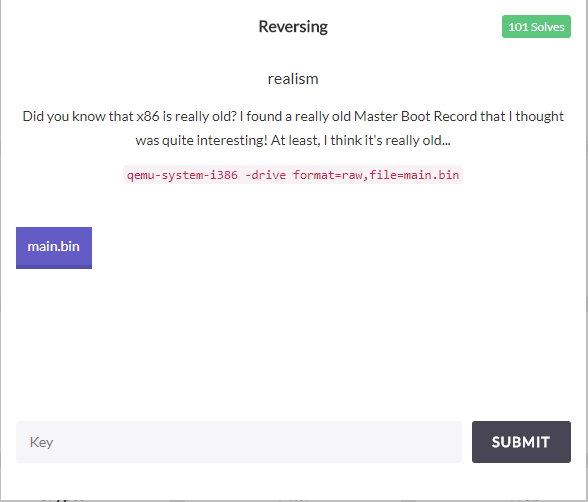
\includegraphics[width=\textwidth]{re400}}
    \end{columns}
\end{frame}

\begin{frame}{A place to start\ldots}
    \begin{columns}
        \column{0.5\textwidth}
	        \begin{itemize}
                \item<1-> Wikipedia, of course!
		        \begin{itemize}
    	            \item<2-> 512 bytes
        	        \item<2-> MBR signature: 55 AA
            	    \item<2-> "expected to contain real mode machine language instructions"
                	\item<2-> little-endian
                	\item<2-> loads at 0000:7C00
	            \end{itemize}                	
            \end{itemize}
        \column{0.5\textwidth}
                {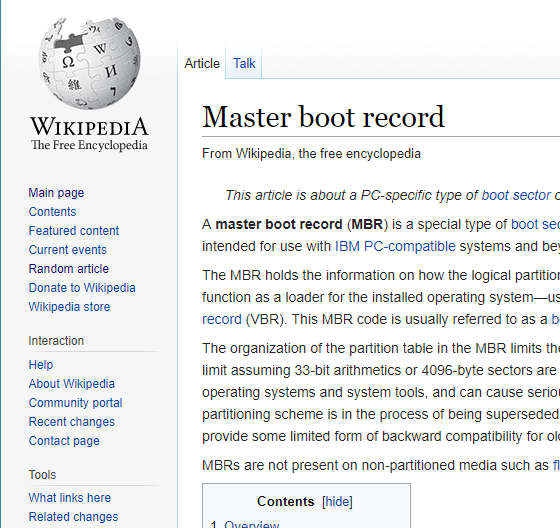
\includegraphics[width=\textwidth]{wikimbr}}
    \end{columns}
\end{frame}

\begin{frame}{Tool Time!\ldots}
    \framesubtitle{qemu (gift wrapped)}
    \begin{columns}
        \column{0.5\textwidth}
            \only<1> {
              	\begin{itemize}
             		\item -s (gdb)
                	\item -S (suspend)
        	       	\item -vnc:1
	            \end{itemize}
            }
            \only<2> {
             	\begin{itemize}
            		\item QEMU/Monitor
              		\begin{itemize}
	    	        	\item info registers
    	    	       	\item system reset
    	    	    \end{itemize}
        	    \end{itemize}
        	}
        \column{0.5\textwidth}
            \only<1>{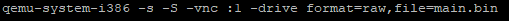
\includegraphics[width=\textwidth]{launch-qemu}\newline\newline
            		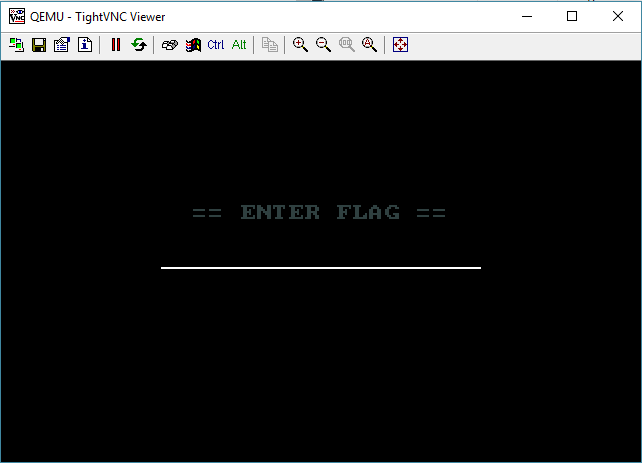
\includegraphics[width=\textwidth]{qemu-vnc}
			}
            \only<2>{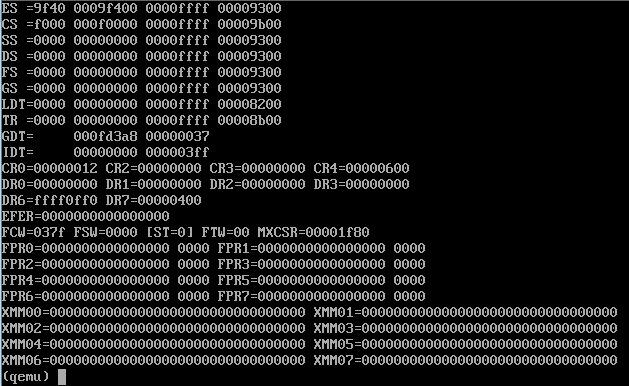
\includegraphics[width=\textwidth]{qemu-info-registers-1}}
    \end{columns}
\end{frame}

\begin{frame}{Tool Time!\ldots}
    \framesubtitle{gdb}
    \begin{columns}
        \column{0.5\textwidth}
                \begin{itemize}
                	\only<1>{
						\item target remote localhost:1234
						\item set architecture i8086
							(bootloaders are 16 bit, right?)
						\item display/i \$pc - print program counter
						\item br *0xADDR - set breakpoint
						\item si - run one instruction
						\item c - continue
					}
					\only<2->{
						\item info reg
						\uncover<3->{\item info frame}
						\uncover<4->{\item x /CT 0xADDR - display C units of T type from ADDR
									\item set {int}0xADDR = 42
									\item set {char[4]} 0xADDR = "AAA"
						}
					}
				\end{itemize}
		\column{0.5\textwidth}
				\only<1>{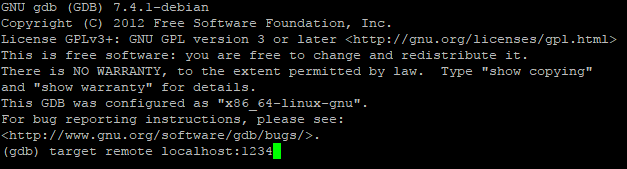
\includegraphics[width=\textwidth]{launch-gdb}\newline\newline
						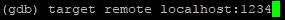
\includegraphics[width=\textwidth]{gdb-target}}
				\only<2>{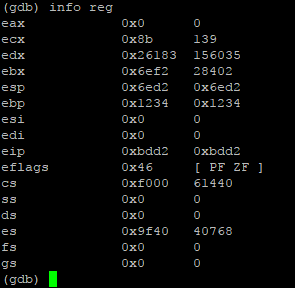
\includegraphics[width=\textwidth]{gdb-info-reg-1}}
				\only<3>{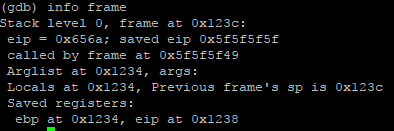
\includegraphics[width=\textwidth]{gdb-info-frame}}
				\only<4-5>{
					\uncover<4->{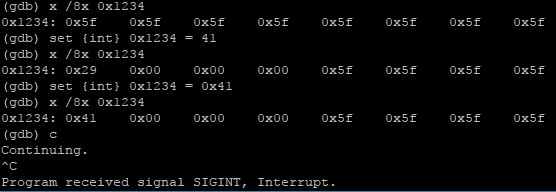
\includegraphics[width=\textwidth]{gdb-x-set-1}}
					\uncover<5->{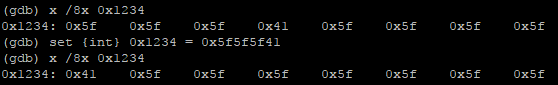
\includegraphics[width=\textwidth]{gdb-x-set-2}}
				}
				\only<6>{
					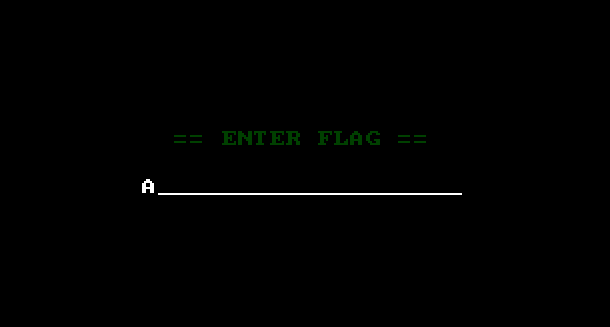
\includegraphics[width=\textwidth]{after-set}
				}
	\end{columns}
\end{frame}